\section{Part 3 --- RL Post-Training Baseline on GSM8K}

\subsection{Results}

In this part, we reproduced the GSM8K RL post-training setup from Karpathy's original \texttt{nanochat} implementation, starting from our Part 2 SFT checkpoint. The training followed the \texttt{nanochat} RL pipeline, which uses on-policy policy-gradient updates with a sparse binary correctness reward and a simple group-mean baseline. The run completed all 467 steps and produced the final checkpoint \texttt{a4p3-rl-baseline@466}.

At the end of training, the final logged step reported an average reward of \textbf{0.3789} and an average sequence length of \textbf{147.71}. These values suggest that the model continued to receive useful reward signal throughout training and did not collapse during optimization.

\begin{figure}[h]
    \centering
    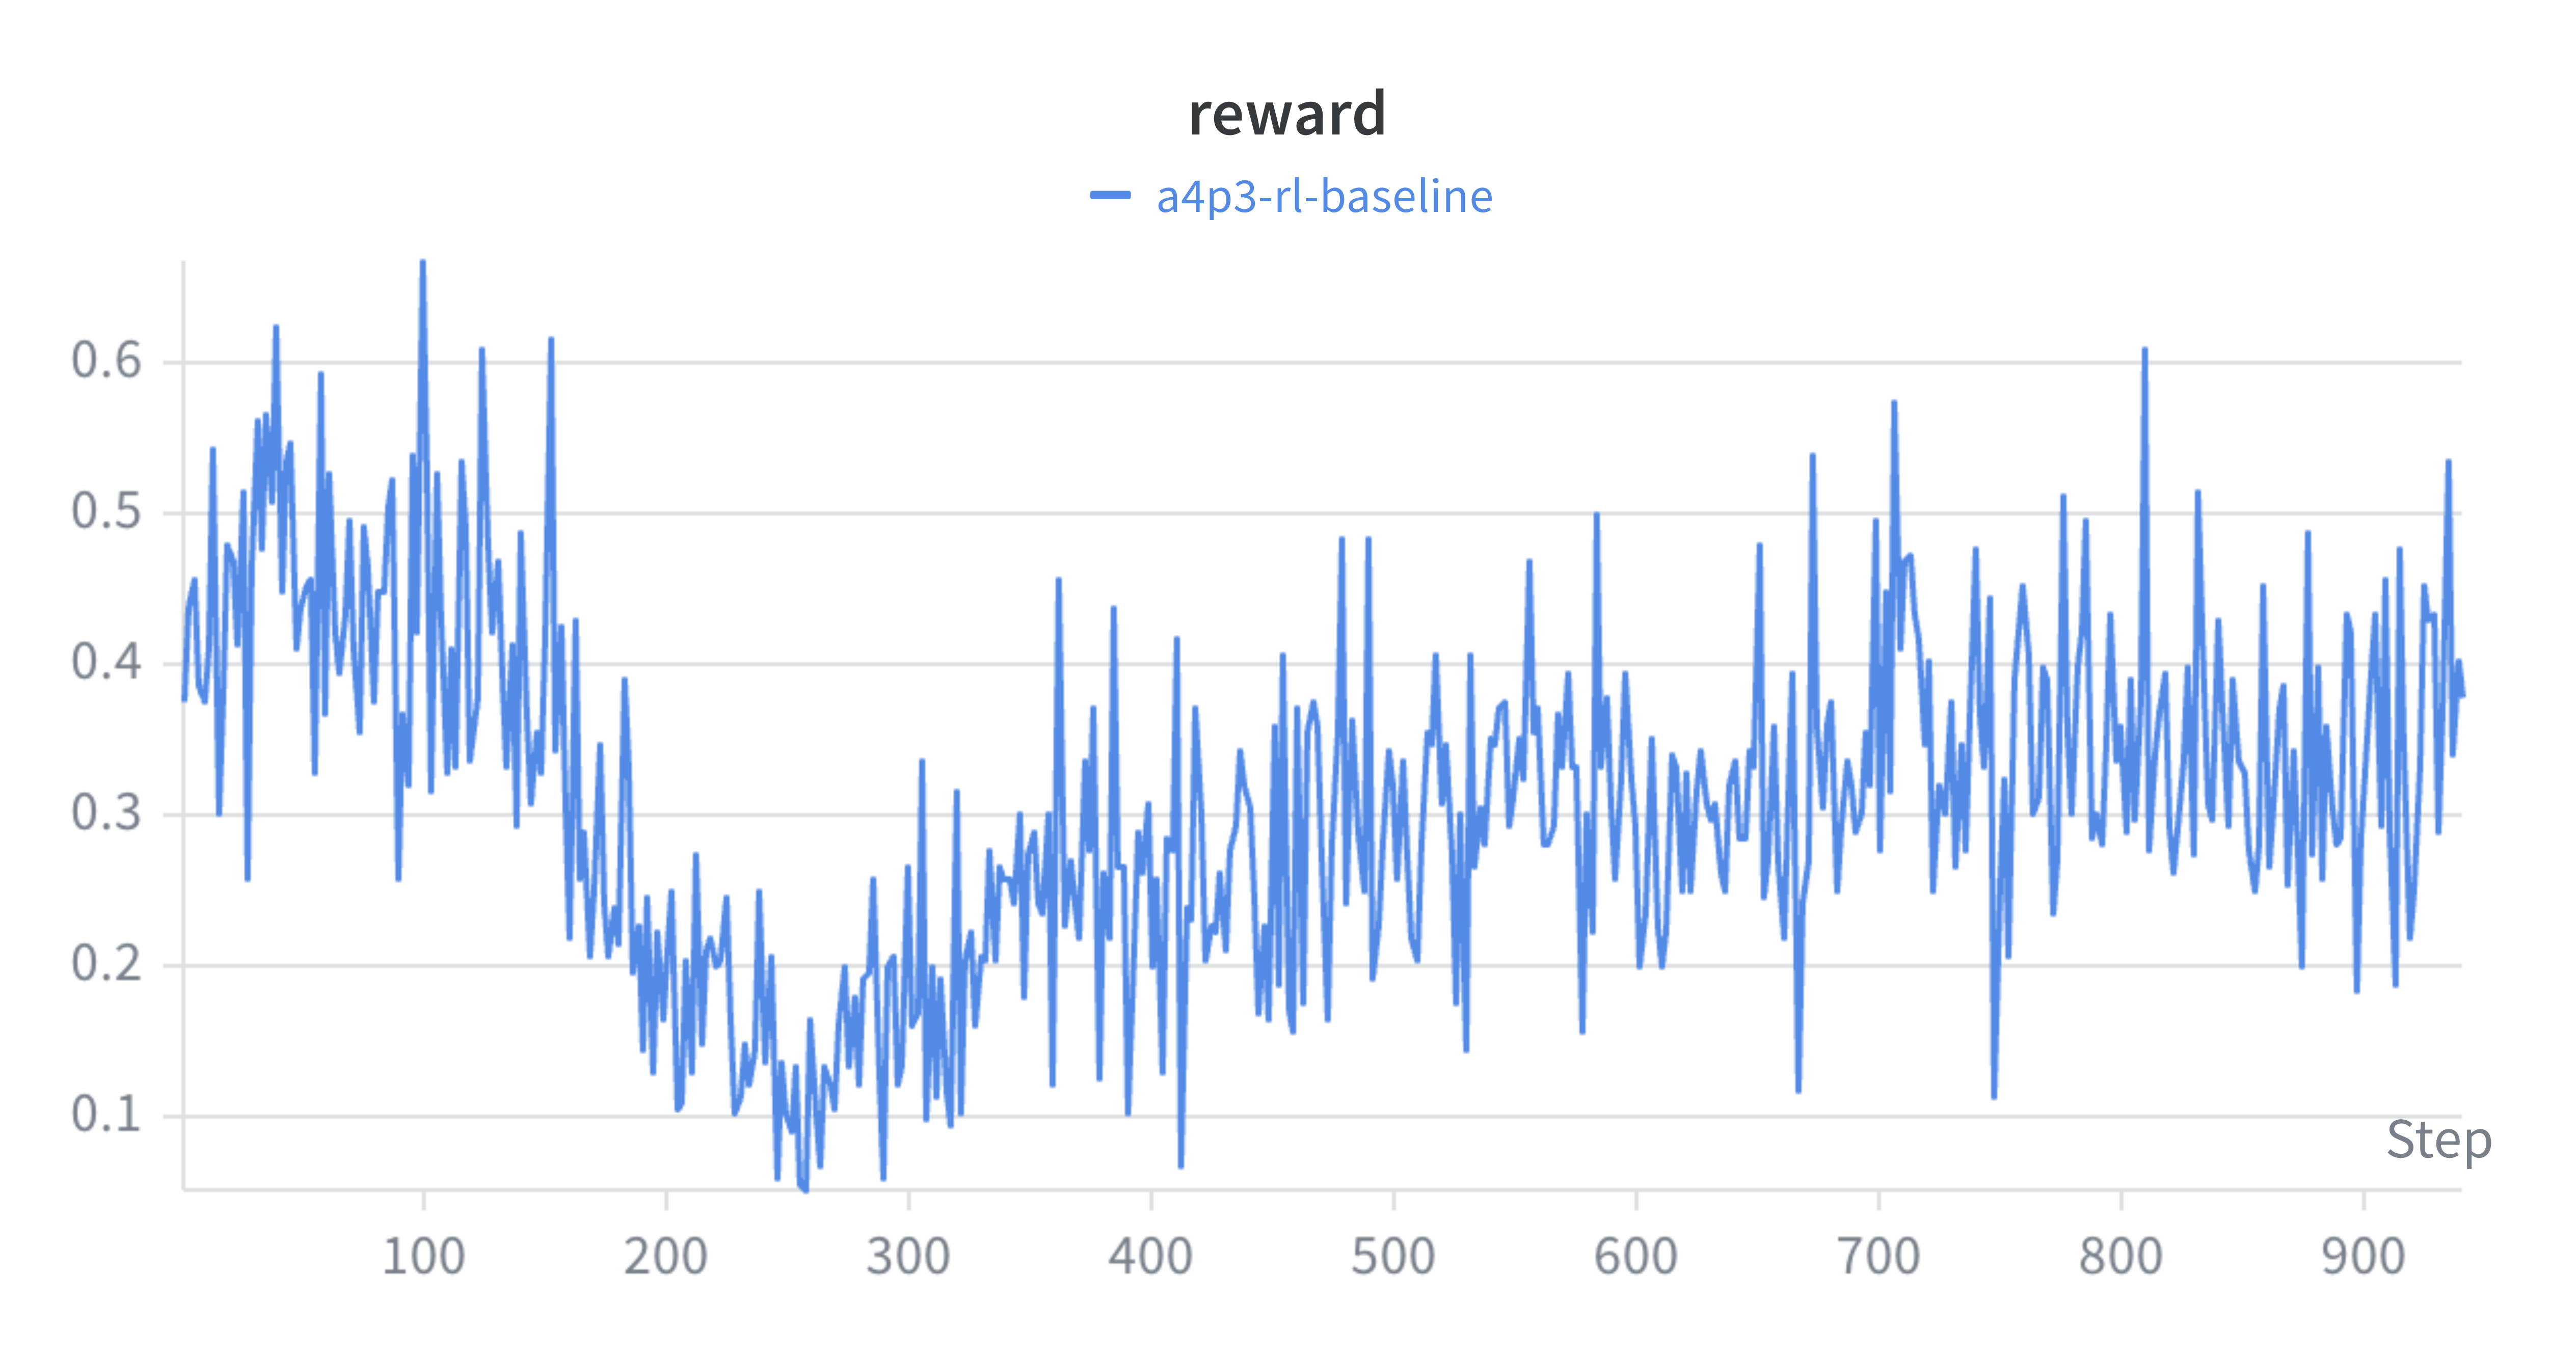
\includegraphics[width=0.8\textwidth]{component/figures/p3/reward.png}
    \caption{Mean reward vs.\ training step for our RL run.}
    \label{fig:p3_reward_curve}
\end{figure}

\begin{figure}[h]
    \centering
    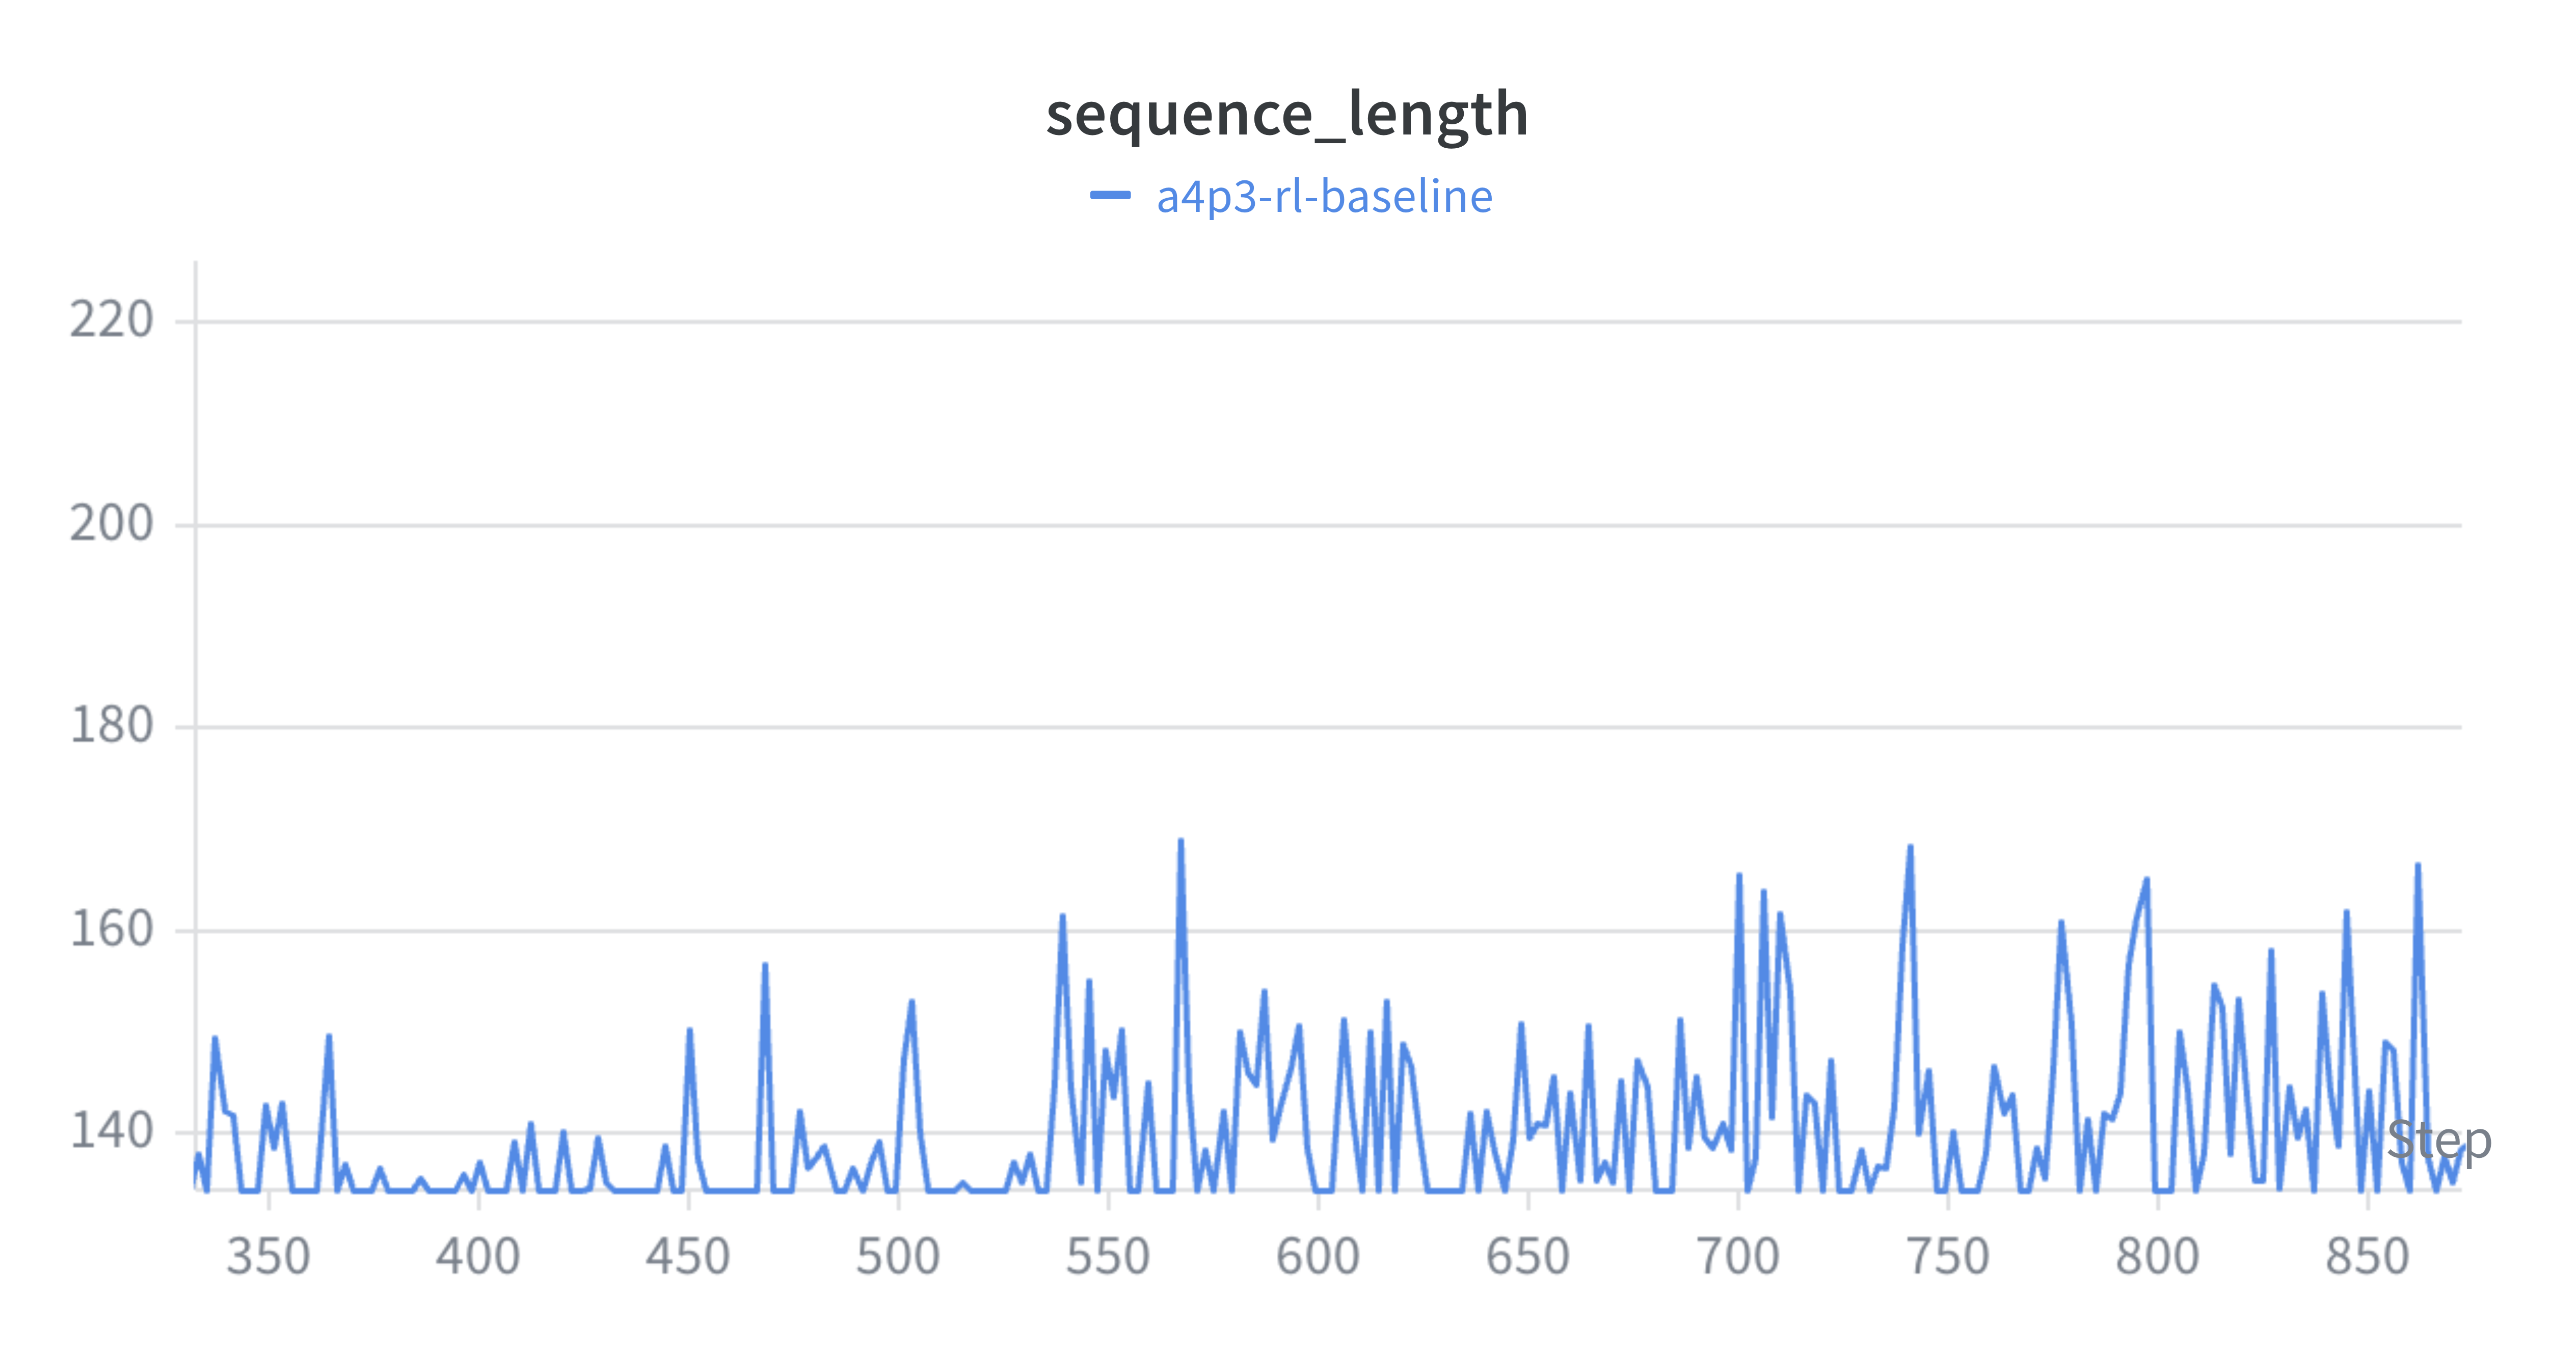
\includegraphics[width=0.8\textwidth]{component/figures/p3/sequence_length.png}
    \caption{Mean sequence length vs.\ training step for our RL run.}
    \label{fig:p3_seq_len_curve}
\end{figure}

\begin{figure}[h]
    \centering
    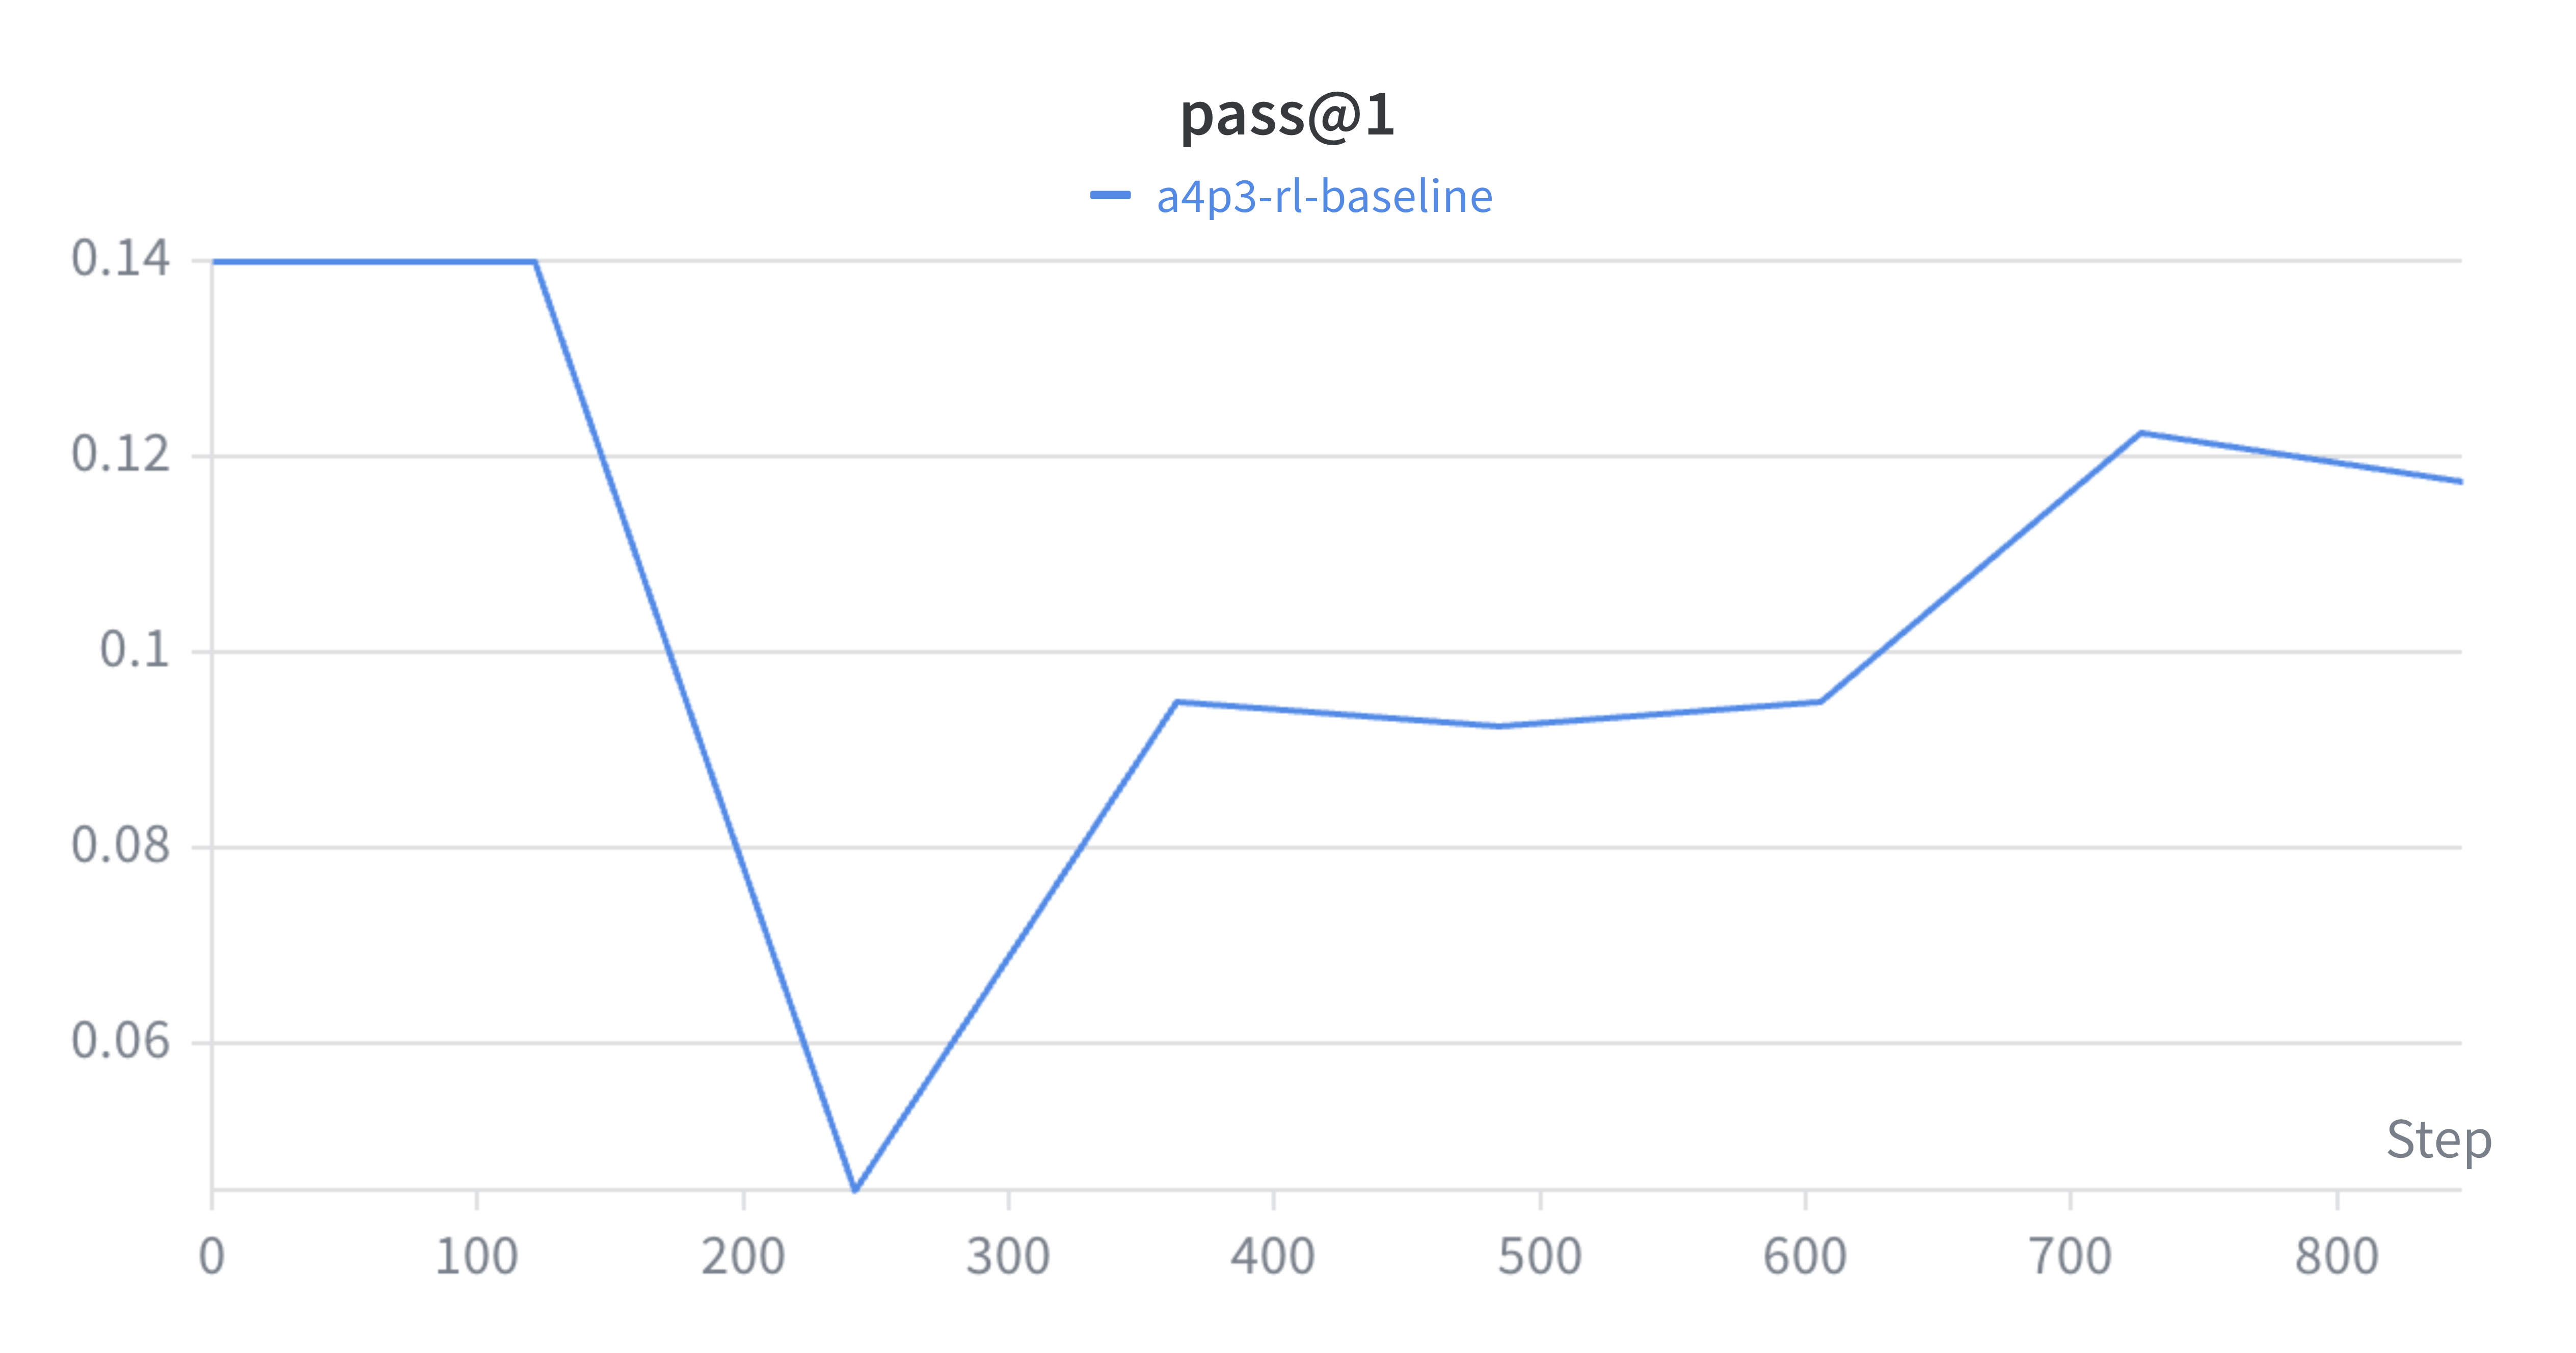
\includegraphics[width=0.8\textwidth]{component/figures/p3/pass1.png}
    \caption{Online evaluation curve(s) during training for our RL run.}
    \label{fig:p3_online_eval_curve}
\end{figure}

We then evaluated the final checkpoint on the full 1,319-problem GSM8K test set. The evaluation produced the following results:

\begin{itemize}
    \item \textbf{Strict accuracy: 17.89\%}
    \item \textbf{Relaxed accuracy: 18.04\%}
    \item \textbf{BPB: 3.4418}
\end{itemize}

These full-set evaluation results are the main basis for our conclusions, since training-time curves are diagnostic only.

\subsection{Comparison with the Original Karpathy Run}

We compare our RL baseline against Karpathy’s original public \texttt{nanochat} RL reference run as documented in GitHub Discussion \#1. In that discussion, Karpathy describes the RL stage as a GSM8K-specific fine-tuning phase run with \texttt{scripts.chat\_rl}, followed by evaluation with \texttt{scripts.chat\_eval -- -i rl -a GSM8K}. He explains that this stage uses a highly simplified GRPO-style loop: it removes trust regions, reference-model KL regularization, and PPO ratio clipping, while using an on-policy update with a reward-shift-by-mean advantage, making it closely aligned with the correctness-only RL setup reproduced in our Part 3 run.  \href{https://github.com/karpathy/nanochat/discussions/1}{GitHub}

Karpathy further notes that the default RL stage is restricted to GSM8K, is not yet fully tuned, and takes about 1.5 hours under the public speedrun setting. The discussion includes a public training figure showing that reward increases over time, while both pass@1 and pass@8 also improve during RL. He also remarks that pass@8 is substantially larger than pass@1, suggesting that repeated sampling yields noticeably better success than single-sample decoding.  
Our Part 3 run exhibits the same broad qualitative pattern. During training, reward rose steadily, the online evaluation curves were generally upward-trending, and the final checkpoint completed all 467 steps without collapse. In this sense, our run is qualitatively consistent with the original public \texttt{nanochat} RL reference: both runs show that correctness-only RL on GSM8K can produce measurable learning signal during post-training.  

At the same time, this comparison should be interpreted as qualitative rather than strictly numerical. The GitHub discussion provides the original RL curve as a public image and a textual description, but not a full downloadable training history with exactly matched logging fields. Therefore, figures 12-14 should be read as visual comparisons between our run and Karpathy’s published reference curves, not as exact point-by-point overlays. Final quantitative conclusions should instead rely on our own full GSM8K post-training evaluation.  

One additional difference is that Karpathy’s public report card summarizes the RL-stage GSM8K result as 0.0758 in the speedrun report, whereas our final checkpoint achieved 17.89\% strict accuracy and 18.04\% relaxed accuracy under our evaluation pipeline. Because the reporting formats are not identical, this number should be treated as a rough public reference rather than a perfectly matched baseline.  

\begin{table}[h]
\centering
\caption{Final comparison of our RL run and Karpathy's public \texttt{nanochat} RL reference run.}
\label{tab:p3_final_comparison}
\begin{tabular}{l l l l}
\hline
\textbf{Model / Stage} & \textbf{Checkpoint} & \textbf{Main Eval Metric(s)}\\
\hline
Karpathy public RL reference & UNSPECIFIED & GSM8K = 0.0758  \\
Our RL run & \texttt{a4p3-rl-baseline@466} & Strict = 17.89\%, Relaxed = 18.04\%  \\
\hline
\end{tabular}
\end{table}


\begin{figure}[h]
    \centering
    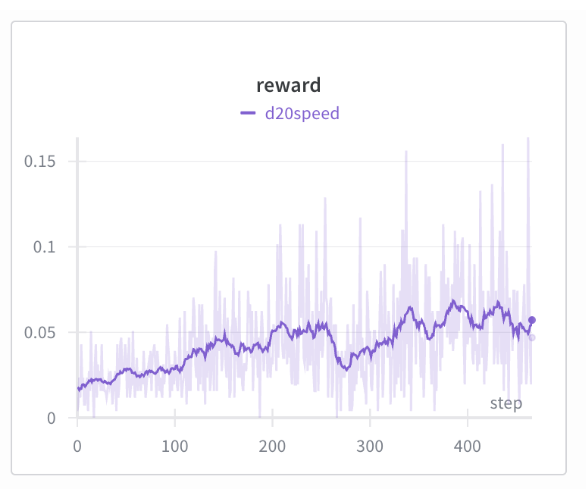
\includegraphics[width=0.8\textwidth]{component/figures/p3/karpathy-reward.png}
    \caption{Reward curve from Karpathy's public \texttt{nanochat} RL reference run, reproduced from GitHub Discussion \#1.}
    \label{fig:p3_karpathy_reward}
\end{figure}

\begin{figure}[H]
    \centering
    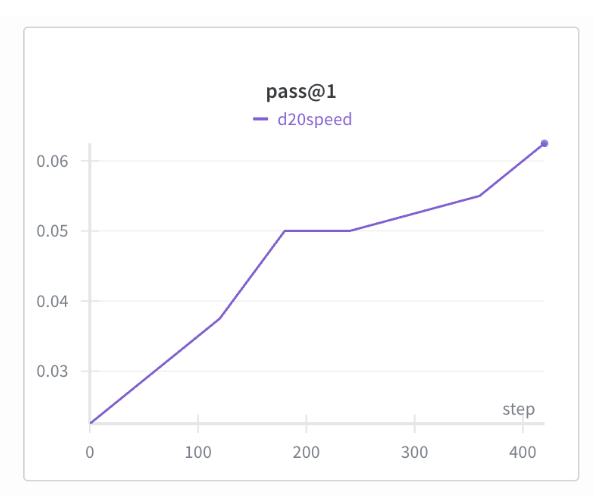
\includegraphics[width=0.8\textwidth]{component/figures/p3/karpathy-pass1.png}
    \caption{Evaluation curves (pass@1) from Karpathy's public \texttt{nanochat} RL reference run, reproduced from GitHub Discussion \#1.}
    \label{fig:p3_karpathy_eval1}
\end{figure}

\begin{figure}[H]
    \centering
    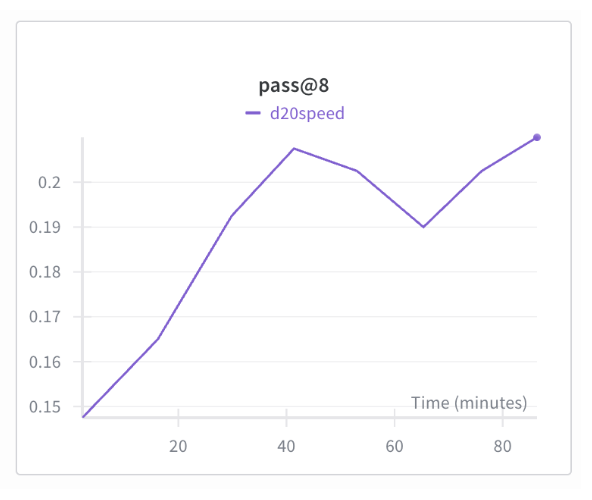
\includegraphics[width=0.8\textwidth]{component/figures/p3/karpathy-pass8.png}
    \caption{Evaluation curves (pass@8) from Karpathy's public \texttt{nanochat} RL reference run, reproduced from GitHub Discussion \#1.}
    \label{fig:p3_karpathy_eval8}
\end{figure}

\subsection{Error Analysis}

To better understand the behavior of the RL-trained model, we examined both the final full-set evaluation results and the online pass@k curves observed during training. Rather than treating all incorrect outputs as a single failure type, we grouped model responses into a small set of qualitative categories that reflect different underlying weaknesses.

First, some responses were \textbf{fully correct}, meaning that the model followed a coherent solution path and produced the correct final extracted answer. These examples show that the RL objective is capable of reinforcing useful task behavior. However, the final offline accuracy remains modest, indicating that such success is still relatively limited overall.

Second, a noticeable class of failures consists of \textbf{mostly correct reasoning with an incorrect final answer}. In these cases, the model often appears to understand the setup of the problem and follows a plausible chain of reasoning, but makes an arithmetic, bookkeeping, or transcription mistake near the end. This type of error is especially important because it suggests that some failures are not caused by total misunderstanding, but by instability in the final stages of generation.

Third, there are \textbf{partial reasoning failures}, where the model identifies relevant quantities or the right general approach but does not complete the derivation successfully. These responses are neither fully random nor fully correct; instead, they indicate incomplete problem solving. This category is consistent with a model that has acquired some problem-specific structure but still lacks reliable end-to-end execution.

Fourth, some failures are best described as \textbf{format or extraction failures}. Since GSM8K correctness in this pipeline depends on extracting a final answer in the expected form, responses that omit or corrupt the final answer marker can be scored as incorrect even if parts of the reasoning are sensible. This matters because some apparent performance gain under RL may come from better alignment with the evaluator's expected answer format rather than from a large improvement in underlying mathematical reasoning alone.

Finally, there are \textbf{degenerate or irrelevant outputs}, including drifting, repetitive, or off-task responses. These failures are less frequent than ordinary reasoning mistakes, but they remain important because they reflect the instability of correctness-only RL without additional regularization or structure.

The online pass@k curves provide additional evidence for this interpretation. During training, all pass@k metrics initially dropped sharply around the early-middle stage of training and then partially recovered. By the end of training, higher-k metrics such as pass@6, pass@7, and pass@8 remained substantially above pass@1, while pass@1 itself recovered only modestly. This pattern suggests that the model often succeeds only under repeated sampling rather than through reliable single-sample reasoning. In other words, RL appears to improve the probability of producing a correct answer somewhere in the sample set, but not yet enough to make the model consistently correct on the first try.

Taken together, these patterns suggest that the main weakness of the Part 3 baseline is not simply the absence of any useful learning signal. The model clearly does learn something under correctness-only RL, as shown by nontrivial reward values and recovering pass@k trends. However, its gains are still limited by a combination of final-step arithmetic errors, incomplete reasoning, format sensitivity, and sample-to-sample instability. 

\subsection{Discussion}

Overall, Part 3 shows that RL post-training on GSM8K can improve performance beyond the earlier reproduced Karpathy baseline, but the improvement is still limited in absolute terms. The final model remains far from robust mathematical reasoning performance, and the gap between encouraging training curves and modest final offline accuracy suggests that correctness-only RL is not sufficient on its own.

This makes Part 3 a useful baseline for Part 4. In particular, Part 4 should test whether additional reward design can improve not only correctness, but also stability, formatting reliability, and consistency across samples.